\section{printpreview.cpp File Reference}
\label{printpreview_8cpp}\index{printpreview.cpp@{printpreview.cpp}}
{\tt \#include $<$QAbstract\-Scroll\-Area$>$}\par
{\tt \#include $<$QPrint\-Dialog$>$}\par
{\tt \#include $<$QPrinter$>$}\par
{\tt \#include $<$QTool\-Bar$>$}\par
{\tt \#include $<$QAction$>$}\par
{\tt \#include $<$QText\-Format$>$}\par
{\tt \#include $<$QMouse\-Event$>$}\par
{\tt \#include $<$QText\-Frame$>$}\par
{\tt \#include $<$QText\-Document$>$}\par
{\tt \#include $<$QAbstract\-Text\-Document\-Layout$>$}\par
{\tt \#include $<$QScroll\-Bar$>$}\par
{\tt \#include $<$QPainter$>$}\par
{\tt \#include $<$QDebug$>$}\par
{\tt \#include $<$QPage\-Setup\-Dialog$>$}\par
{\tt \#include $<$QStatus\-Bar$>$}\par
{\tt \#include \char`\"{}printpreview.h\char`\"{}}\par
{\tt \#include \char`\"{}printpreview.moc\char`\"{}}\par


Include dependency graph for printpreview.cpp:\begin{figure}[H]
\begin{center}
\leavevmode
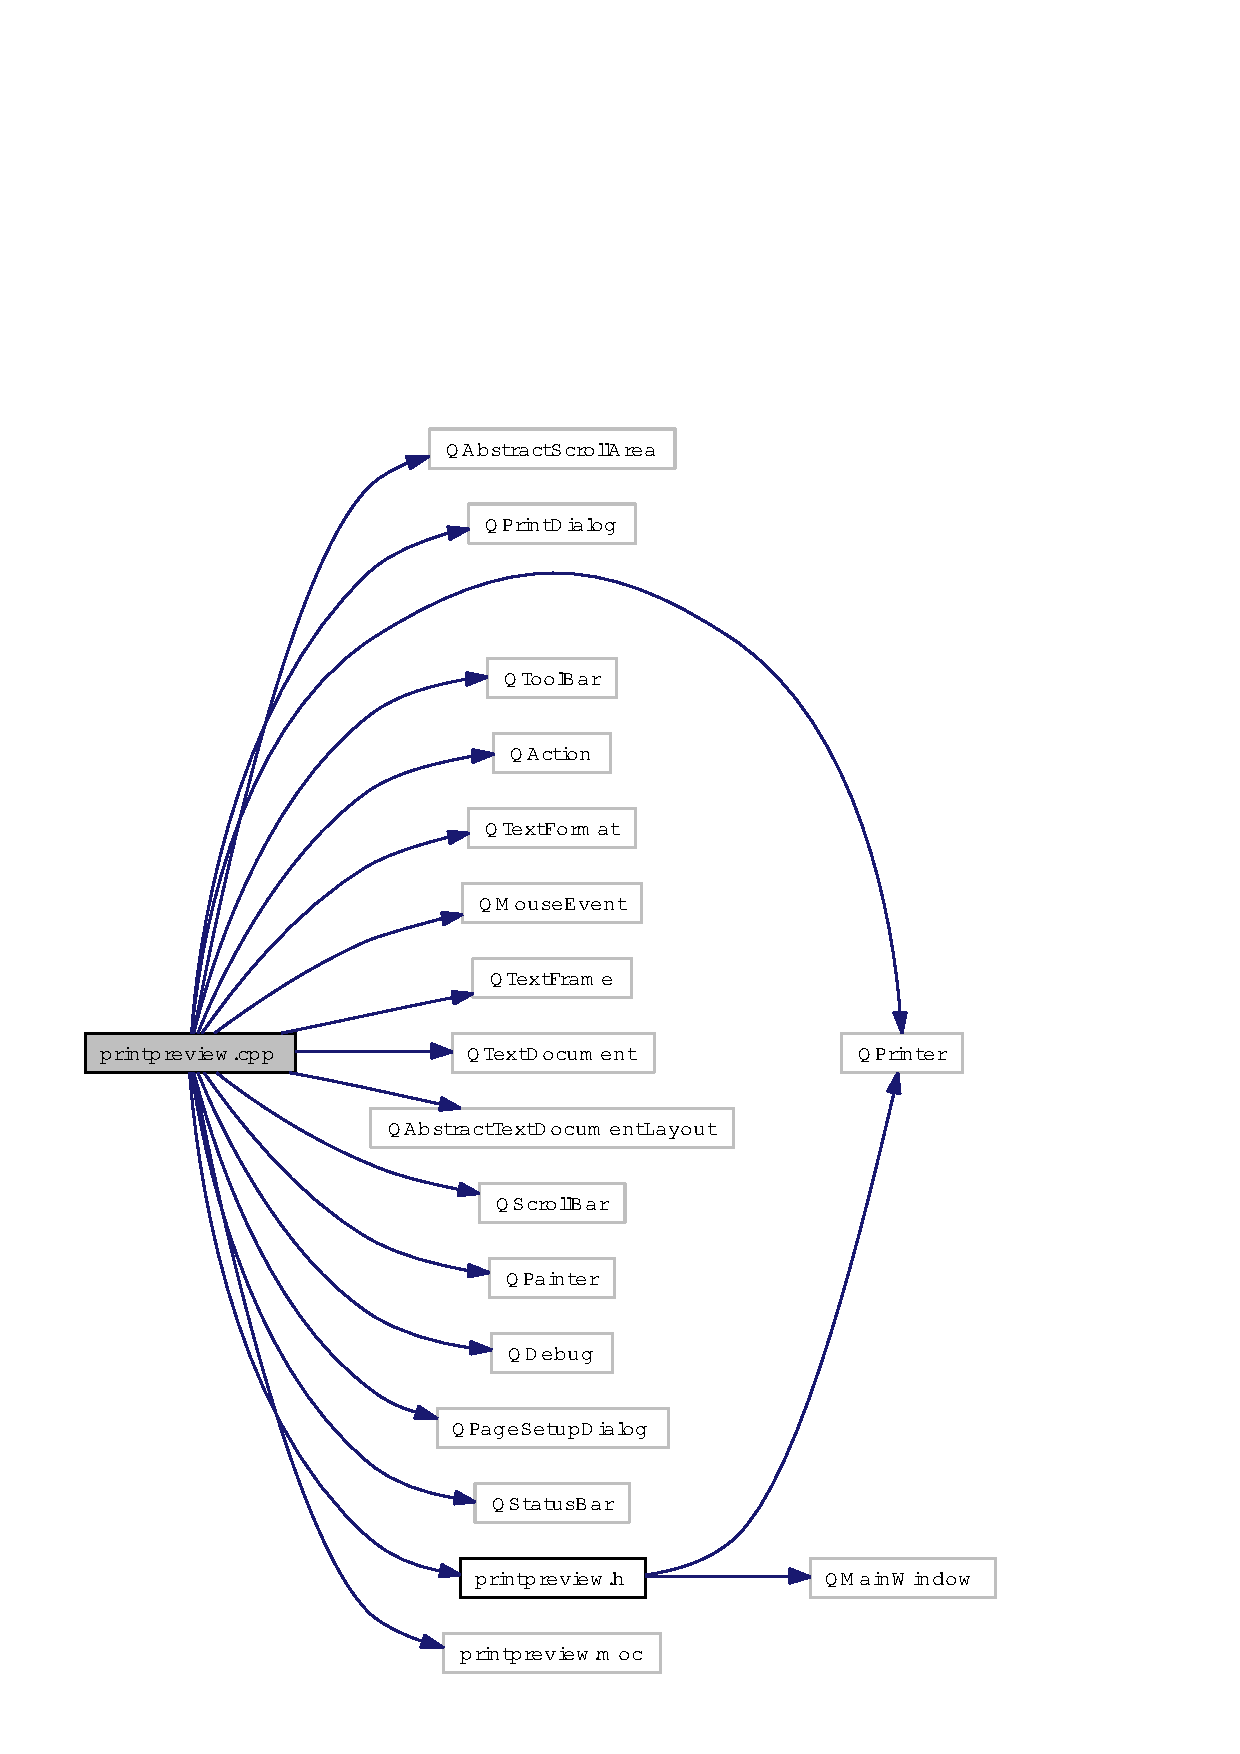
\includegraphics[width=241pt]{printpreview_8cpp__incl}
\end{center}
\end{figure}
\subsection*{Classes}
\begin{CompactItemize}
\item 
class {\bf Preview\-View}
\end{CompactItemize}
\subsection*{Functions}
\begin{CompactItemize}
\item 
static int {\bf inches\-To\-Pixels} (float inches, QPaint\-Device $\ast$device)
\item 
static qreal {\bf mm\-To\-Inches} (double mm)
\end{CompactItemize}
\subsection*{Variables}
\begin{CompactItemize}
\item 
const QString {\bf rsrc\-Path} = \char`\"{}:/images/win\char`\"{}
\end{CompactItemize}


\subsection{Function Documentation}
\index{printpreview.cpp@{printpreview.cpp}!inchesToPixels@{inchesToPixels}}
\index{inchesToPixels@{inchesToPixels}!printpreview.cpp@{printpreview.cpp}}
\subsubsection{\setlength{\rightskip}{0pt plus 5cm}static int inches\-To\-Pixels (float {\em inches}, QPaint\-Device $\ast$ {\em device})\hspace{0.3cm}{\tt  [inline, static]}}\label{printpreview_8cpp_fd6bdb40c251834098e7103dae6b7a0f}




Definition at line 48 of file printpreview.cpp.

Referenced by Print\-Preview::Print\-Preview(), and Print\-Preview::setup().

Here is the caller graph for this function:\begin{figure}[H]
\begin{center}
\leavevmode
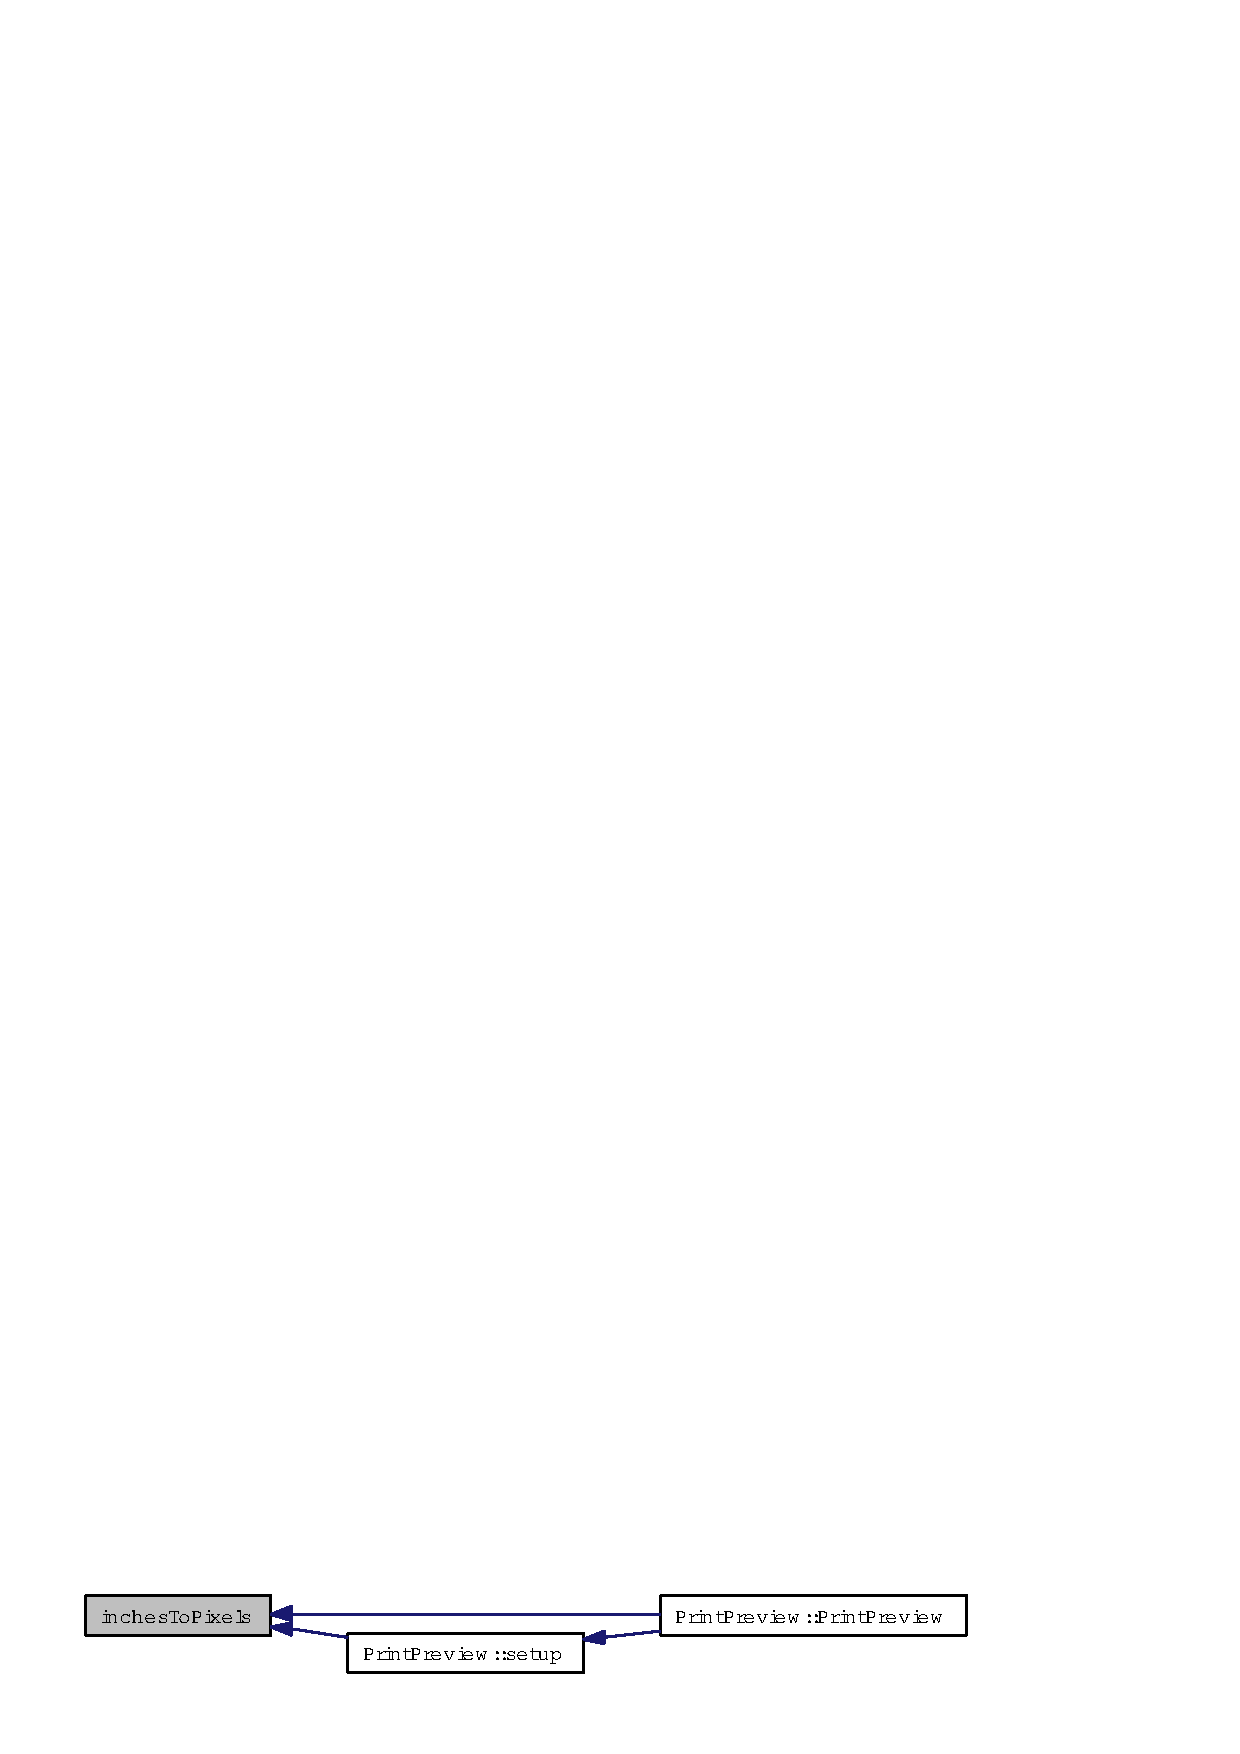
\includegraphics[width=234pt]{printpreview_8cpp_fd6bdb40c251834098e7103dae6b7a0f_icgraph}
\end{center}
\end{figure}
\index{printpreview.cpp@{printpreview.cpp}!mmToInches@{mmToInches}}
\index{mmToInches@{mmToInches}!printpreview.cpp@{printpreview.cpp}}
\subsubsection{\setlength{\rightskip}{0pt plus 5cm}static qreal mm\-To\-Inches (double {\em mm})\hspace{0.3cm}{\tt  [inline, static]}}\label{printpreview_8cpp_09e5069d26dad860da983478e7b29c5e}




Definition at line 53 of file printpreview.cpp.

Referenced by Print\-Preview::Print\-Preview(), and Print\-Preview::setup().

Here is the caller graph for this function:\begin{figure}[H]
\begin{center}
\leavevmode
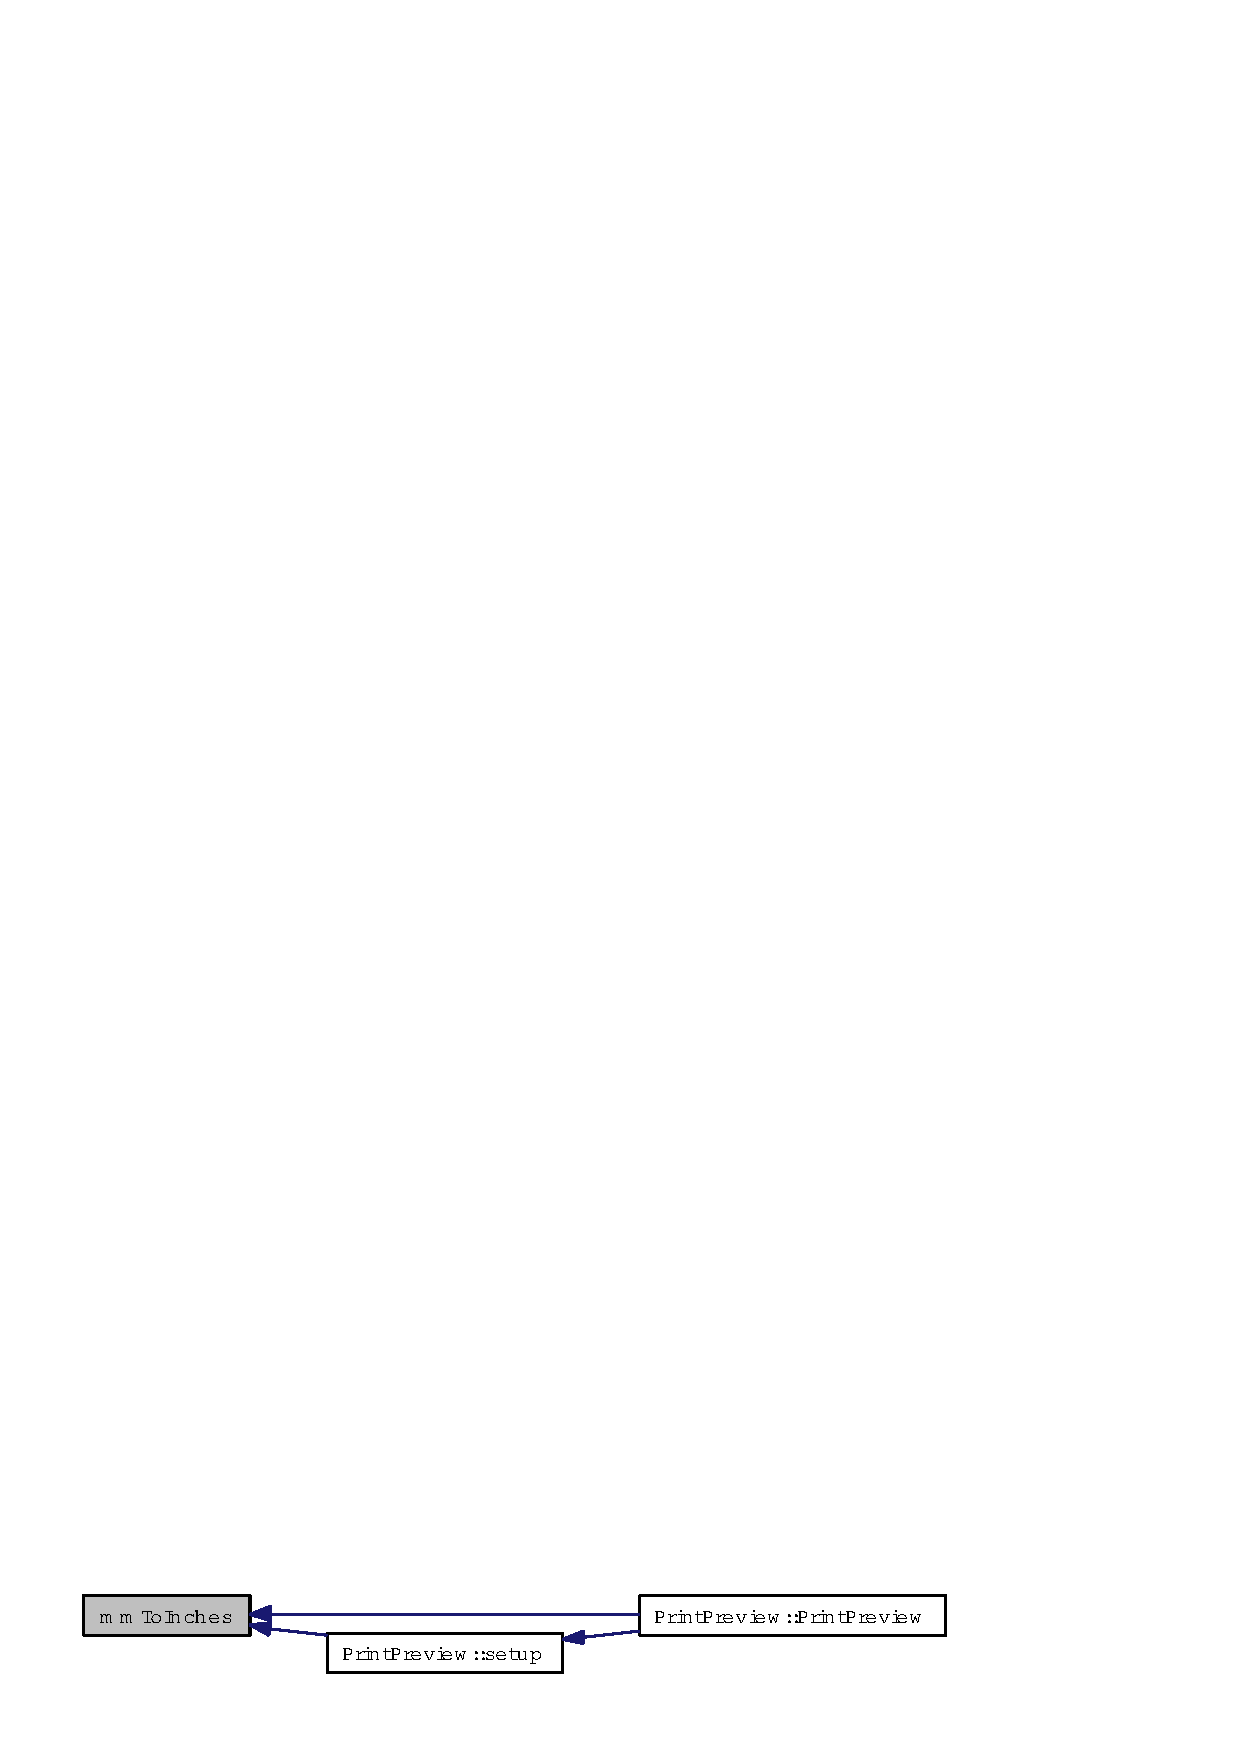
\includegraphics[width=229pt]{printpreview_8cpp_09e5069d26dad860da983478e7b29c5e_icgraph}
\end{center}
\end{figure}


\subsection{Variable Documentation}
\index{printpreview.cpp@{printpreview.cpp}!rsrcPath@{rsrcPath}}
\index{rsrcPath@{rsrcPath}!printpreview.cpp@{printpreview.cpp}}
\subsubsection{\setlength{\rightskip}{0pt plus 5cm}const QString {\bf rsrc\-Path} = \char`\"{}:/images/win\char`\"{}}\label{printpreview_8cpp_48f57ebe9b64d55d98423f57eda3e6bb}




Definition at line 45 of file printpreview.cpp.